\subsubsection{Suite}\label{Testing:About:Suite}
	In this section we will talk about the testing suite and how it works and what is does.
	
	Since we chose to do most of our testing on NS3 using the MobiEmu\footnote{A framework for emulating mobile ad-hoc networks with Linux containers and ns-3. \url{https://code.google.com/p/mobiemu/}} framework most of our tests are fully automated. As we have not manage to integrate everything into the testing framework some variables are still static, but these will be highlighted where applicable.

	\begin{shaded}
	Please refer to appendix \ref{Mobiemu Setup Guide} for instruction on how to set up the testing framework. And for a description of the different variables in the test.
	\end{shaded}
	
	As we alluded to in section \ref{System testing} we had quite high hopes for how we were going to test the whole system. Unfortunately for us that did not pan out the way we wanted it to. We had some major problems regarding NS3 and how it connects its nodes to the Tap-Bridges created. This led us to having to rethink our whole test setup. We decided, after talking to the customer, that we would change the test and create a simpler network layout which would work with NS3. In figure: \ref{fig:NS3network} you can see this new altered network layout. What this means for the project is that we can not test all the functionality that we wanted to, but we are still quietly confident that we can draw some conclusion about the results. In appendix \ref{NS3 Problems} we have outlined the problems we faced and a possible solution that we did not have time to implement.
	
	\begin{figure}[H]
        \centering
        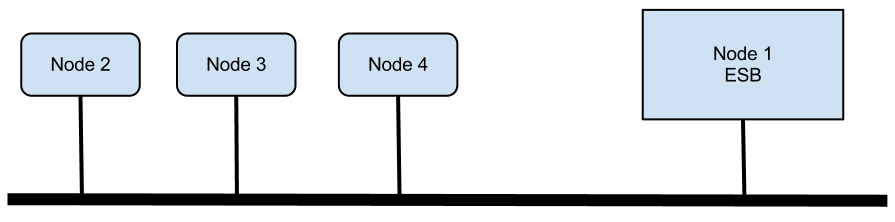
\includegraphics[width=\textwidth, scale=0.3]{NS3network}
        \caption{The layout of our network during testing}
        In this figure we have illustrated the layout of the network during NS3 testing.
        \label{fig:NS3network}
    \end{figure}
    
    This new layout does limit the scope of the test and also what we can approve of functionality, but still we think we have a strong end product with results that will absolutely be relevant for the customer.
    
    
